% ============================================================================
%  COMPILE WITH XeLaTeX  (twice, so the point total resolves)
%  Overleaf: Menu -> Compiler -> XeLaTeX
%  Requires: bnhandout.sty and fonts/Kalpurush.ttf in the project
% ============================================================================
\documentclass[11pt]{article}
\usepackage{bnhandout}          % add [nosol] for a student edition

\hauthor[https://jugantordey.github.io/]{Jugantor Dey}
\hseries{\textit{Mathematics for the Physics Olympiad}}

\begin{document}

\handouttitle{Chapter 9 : Inequalities}

\noindent
শুরু করার আগে ৩ নম্বর অধ্যায় থেকে পূর্ণবর্গ সম্পূর্ণ করা আর $a^2 - b^2$
ধরনের অভেদগুলো, এবং ৮ নম্বর অধ্যায় থেকে ভগ্নাংশ সূচক, $n$-তম মূল ও সিগমা
নোটেশন একবার ঝালিয়ে নাও। এই দুটোই এখানে সারাক্ষণ লাগবে।

এতদিন তুমি সমীকরণ সমাধান করে এসেছ, অর্থাৎ কোন কোন মানের জন্য দুই পক্ষ ঠিক সমান
হয় তা খুঁজেছ। অসমতার প্রশ্নটা আলাদা: একটি রাশি কত বড় বা কত ছোট হতে পারে, সেটা
জানতে চাওয়া। ভৌত সমস্যায় বহুবার দেখা যায় যে সঠিক মান বের করা কঠিন, অথচ মানটি
কোন সীমার ভেতরে থাকতেই হবে তা সহজেই বলা যায়; আর অনেক সময় ওই সীমাটুকুই যথেষ্ট।
আরও মজার ব্যাপার হলো, অসমতা দিয়ে ক্যালকুলাস ছাড়াই কিছু চরম মান (maximum ও
minimum) হুবহু নির্ণয় করা যায়, যা আমরা শেষ অনুচ্ছেদে করব।

এখানে একটি নতুন প্রমাণকৌশলও শেখানো হবে: গাণিতিক আরোহ বা mathematical induction।
আগের কোনো অধ্যায়ে এটি আসেনি, তাই AM--GM অসমতার সাধারণ রূপ প্রমাণ করার ঠিক
আগে সেটিকে আলাদা করে দাঁড় করানো হয়েছে। এই অধ্যায়ে মোট \totalpoints\
পয়েন্ট আছে।

\section{অসমতার নিয়ম}

সমীকরণে যা যা করা যায়, অসমতাতেও প্রায় তার সবই করা যায়; একটিমাত্র জায়গা ছাড়া।
সেই একটি জায়গাই বেশিরভাগ ভুলের উৎস, তাই নিয়মগুলো একদম গোড়া থেকে বসিয়ে নিই।

সংজ্ঞা: $a < b$ লেখার অর্থ $b - a$ একটি ধনাত্মক সংখ্যা। এই একটি বাক্য থেকেই
নিচের সব নিয়ম বেরিয়ে আসে, কারণ ধনাত্মক সংখ্যা সম্পর্কে আমরা মাত্র দুটো জিনিস
ধরে নিচ্ছি: দুটি ধনাত্মক সংখ্যার যোগফল ধনাত্মক, এবং দুটি ধনাত্মক সংখ্যার গুণফল
ধনাত্মক।

\begin{idea}[অসমতার মৌলিক নিয়ম]
$a, b, c, d$ বাস্তব সংখ্যা হলে:
\begin{enumerate}
  \item $a < b$ হলে $a + c < b + c$ (যেকোনো $c$-এর জন্য)।
  \item $a < b$ এবং $c < d$ হলে $a + c < b + d$।
  \item $a < b$ এবং $c > 0$ হলে $ac < bc$।
  \item $a < b$ এবং $c < 0$ হলে $ac > bc$ (চিহ্ন উল্টে যায়)।
  \item $0 < a < b$ হলে $\dfrac{1}{a} > \dfrac{1}{b}$।
  \item $0 < a < b$ এবং $0 < c < d$ হলে $ac < bd$।
  \item যেকোনো বাস্তব $x$-এর জন্য $x^2 \geq 0$, এবং সমতা কেবল $x = 0$-এ।
\end{enumerate}
\end{idea}

তিন ও চার নম্বর নিয়মের প্রমাণ একই লাইনে হয়ে যায়: $bc - ac = (b-a)c$। এখানে
$b - a$ ধনাত্মক। তাই $c$ ধনাত্মক হলে গুণফল ধনাত্মক, অর্থাৎ $ac < bc$; আর $c$
ঋণাত্মক হলে গুণফল ঋণাত্মক, অর্থাৎ $ac > bc$। পাঁচ নম্বর নিয়মও একইভাবে:
\[
  \frac{1}{a} - \frac{1}{b} \;=\; \frac{b-a}{ab},
\]
যার লব ধনাত্মক এবং হর ধনাত্মক, সুতরাং পুরোটা ধনাত্মক।

সাত নম্বর নিয়মটি দেখতে তুচ্ছ, কিন্তু এই গোটা অধ্যায়ের প্রায় প্রতিটি প্রমাণ
শেষ পর্যন্ত এটির উপরেই দাঁড়ানো। কোনো অসমতা প্রমাণ করতে বললে প্রথম চেষ্টা হওয়া
উচিত: সবকিছু এক পাশে নিয়ে গিয়ে দেখা যায় কি না যে অবশিষ্টটা আসলে একটি বর্গের
যোগফল।

\begin{remark}
যা \emph{করা যায় না}, সেটাও একইরকম গুরুত্বপূর্ণ। দুটি অসমতা যোগ করা যায়, কিন্তু
\emph{বিয়োগ করা যায় না}: $1 < 2$ এবং $0 < 5$ থেকে $1 - 0 < 2 - 5$ পাওয়া যায়
না। একইভাবে দুই পাশে বর্গ করা যায় কেবল তখনই, যখন দুই পাশই অঋণাত্মক: $-3 < 1$
সত্য, কিন্তু $9 < 1$ নয়।
\end{remark}

\begin{example}
$x^2 - 7x + 10 < 0$ অসমতাটি সমাধান করো।
\end{example}

\begin{solbox}
বাম পাশ উৎপাদকে বিশ্লেষণ করি (৩ নম্বর অধ্যায়): $x^2 - 7x + 10 = (x-2)(x-5)$।
দুটি সংখ্যার গুণফল ঋণাত্মক হয় তখনই, যখন তাদের চিহ্ন আলাদা। $x = 2$ ও $x = 5$
বিন্দু দুটি সংখ্যারেখাকে তিন ভাগে ভাগ করে; প্রতিটি ভাগে চিহ্ন দেখে নিই।

\begin{center}
\begin{tabular}{c|c|c|c}
 ব্যবধি & $x-2$ & $x-5$ & $(x-2)(x-5)$ \\ \hline
 $x < 2$     & $-$ & $-$ & $+$ \\
 $2 < x < 5$ & $+$ & $-$ & $-$ \\
 $x > 5$     & $+$ & $+$ & $+$ \\
\end{tabular}
\end{center}

সুতরাং সমাধান $2 < x < 5$, অর্থাৎ ব্যবধি $(2,5)$। প্রান্তবিন্দু দুটি বাদ, কারণ
সেখানে গুণফল $0$, ঋণাত্মক নয়।

\begin{center}
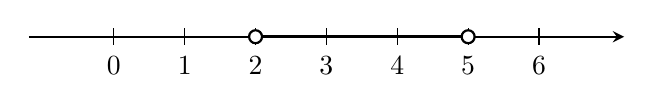
\begin{tikzpicture}[scale=0.9,>=stealth]
  \draw[thick,->] (-1.2,0) -- (7.2,0);
  \foreach \x in {0,1,2,3,4,5,6} \draw (\x,0.12) -- (\x,-0.12);
  \foreach \x in {0,1,2,3,4,5,6} \node[below] at (\x,-0.15) {$\x$};
  \draw[very thick] (2,0) -- (5,0);
  \draw[fill=white,thick] (2,0) circle (2.6pt);
  \draw[fill=white,thick] (5,0) circle (2.6pt);
\end{tikzpicture}
\end{center}
\end{solbox}

\begin{example}
$\dfrac{1}{x-2} < 3$ অসমতাটি সমাধান করো।
\end{example}

\begin{solbox}
এখানে $x - 2$ দিয়ে গুণ করার লোভ হয়, কিন্তু তার চিহ্ন আমরা জানি না। দুটি পথ আছে।

\textbf{পথ ১ (ভাগ করে দেখা)।} $x > 2$ হলে $x - 2 > 0$, তাই গুণ করলে চিহ্ন
অপরিবর্তিত থাকে: $1 < 3(x-2) = 3x - 6$, অর্থাৎ $x > 7/3$। যেহেতু $7/3 > 2$,
এই ক্ষেত্রে শর্ত দাঁড়ায় $x > 7/3$। আবার $x < 2$ হলে $x - 2 < 0$, তাই গুণ করলে
চিহ্ন উল্টে যায়: $1 > 3x - 6$, অর্থাৎ $x < 7/3$; এটি $x < 2$-এর সঙ্গে মিলিয়ে
কোনো নতুন সীমা দেয় না, তাই পুরো $x < 2$ অংশটিই সমাধান।

\textbf{পথ ২ (এক পাশে নিয়ে যাওয়া)।} সব কিছু বাম পাশে এনে
\[
  \frac{1}{x-2} - 3 \;=\; \frac{1 - 3(x-2)}{x-2} \;=\; \frac{7 - 3x}{x-2} \;<\; 0 .
\]
ভগ্নাংশটি ঋণাত্মক হওয়ার শর্ত আর $(7-3x)(x-2) < 0$ হওয়ার শর্ত একই, কারণ হর
$x-2$ দিয়ে ভাগ করা আর $(x-2)^2$ (যা সর্বদা ধনাত্মক) দিয়ে গুণ করা একই কথা।
চিহ্নের ছক করলে পাই $x < 2$ অথবা $x > 7/3$।

দুই পথেই উত্তর এক: $x < 2$ অথবা $x > 7/3$। যাচাই: $x = 0$ দিলে বাম পাশ $-0.5$,
সত্য; $x = 2.2$ দিলে বাম পাশ $5$, মিথ্যা; $x = 3$ দিলে বাম পাশ $1$, সত্য।
\end{solbox}

\begin{remark}
পথ ২-ই অভ্যাস করা ভালো। ভগ্নাংশযুক্ত অসমতায় হর দিয়ে গুণ করতে গিয়ে চিহ্নের
ক্ষেত্রবিভাগ ভুলে যাওয়া এই বিষয়ের সবচেয়ে সাধারণ ভুল। সব এক পাশে নিয়ে গেলে
সেই ফাঁদ এড়ানো যায়, কারণ তখন আর কোনো অজানা-চিহ্নের রাশি দিয়ে গুণ করতে হয় না।
\end{remark}

\prob{2} নিচের অসমতাগুলো সমাধান করে ব্যবধি আকারে লেখো।
\begin{enumerate}
  \item $4x - 3 < 6x + 5$
  \item $x^2 + x > 6$
  \item $-5 \leq 3 - 2x < 7$
\end{enumerate}

\begin{sol}
\begin{enumerate}
  \item $-8 < 2x$, অর্থাৎ $x > -4$; ব্যবধি $(-4, \infty)$।
  \item $x^2 + x - 6 > 0$, অর্থাৎ $(x+3)(x-2) > 0$। চিহ্নের ছক থেকে $x < -3$
        অথবা $x > 2$; ব্যবধি $(-\infty,-3) \cup (2,\infty)$।
  \item তিন পাশ থেকে $3$ বিয়োগ করে $-8 \leq -2x < 4$। এবার $-2$ দিয়ে ভাগ করলে
        দুটি চিহ্নই উল্টে যায়: $4 \geq x > -2$, অর্থাৎ $-2 < x \leq 4$;
        ব্যবধি $(-2, 4]$।
\end{enumerate}
\end{sol}

\prob{2} $\dfrac{2x+1}{x-3} \geq 1$ সমাধান করো।

\begin{sol}
সব এক পাশে নিই:
\[
  \frac{2x+1}{x-3} - 1 \;=\; \frac{2x + 1 - (x-3)}{x-3} \;=\; \frac{x+4}{x-3} \;\geq\; 0 .
\]
ভগ্নাংশটি অঋণাত্মক হওয়ার শর্ত $(x+4)(x-3) \geq 0$, তবে $x = 3$ বাদ দিতে হবে
কারণ সেখানে রাশিটি সংজ্ঞায়িত নয়। সুতরাং সমাধান $x \leq -4$ অথবা $x > 3$।
যাচাই: $x = -4$ দিলে বাম পাশ $\frac{-7}{-7} = 1$, সত্য; $x = 0$ দিলে
$-\frac{1}{3}$, মিথ্যা; $x = 4$ দিলে $9$, সত্য।
\end{sol}

\prob{2} নিচের দাবিগুলো ভুল। প্রতিটির জন্য একটি করে পাল্টা উদাহরণ দাও, এবং
(ক)-এর ক্ষেত্রে দাবিটিকে সত্য করতে কী শর্ত যোগ করা দরকার তা বলো।
\begin{enumerate}
  \item $a < b$ হলে $a^2 < b^2$।
  \item $a < b$ এবং $c < d$ হলে $a - c < b - d$।
\end{enumerate}

\begin{sol}
\begin{enumerate}
  \item $a = -3$, $b = 1$ নিলে $a < b$, কিন্তু $a^2 = 9 > 1 = b^2$। দাবিটি সত্য
        হয় যদি অতিরিক্তভাবে $0 \leq a$ ধরা হয়, অর্থাৎ $0 \leq a < b$ হলে
        $a^2 < b^2$। ($0 < a < b$ হলে নিয়ম ৬-এ $c = a$, $d = b$ বসালেই এটি
        পাওয়া যায়; আর $a = 0$ হলে ফলটি স্পষ্ট।)
  \item $a = 1$, $b = 2$, $c = 0$, $d = 5$ নিলে দুটি শর্তই মানা হয়, কিন্তু
        $a - c = 1$ এবং $b - d = -3$, সুতরাং $a - c < b - d$ মিথ্যা। অসমতা
        যোগ করা যায়, বিয়োগ করা যায় না।
\end{enumerate}
\end{sol}

\prob{3} যেকোনো বাস্তব $a, b, c$-এর জন্য প্রমাণ করো যে
$a^2 + b^2 + c^2 \geq ab + bc + ca$, এবং সমতা কখন ঘটে তা নির্ণয় করো।

\begin{sol}
দুই পাশের পার্থক্য নিয়ে $2$ দিয়ে গুণ করি:
\[
  2(a^2+b^2+c^2) - 2(ab+bc+ca)
  = (a-b)^2 + (b-c)^2 + (c-a)^2 \;\geq\; 0 ,
\]
কারণ ডান পাশ তিনটি বর্গের যোগফল। সুতরাং $a^2+b^2+c^2 \geq ab+bc+ca$। সমতা তখনই,
যখন তিনটি বর্গই শূন্য, অর্থাৎ $a = b = c$।
\end{sol}

\section{AM--GM}

দুটি অঋণাত্মক সংখ্যার গড় দুইভাবে নেওয়া যায়: যোগ করে অর্ধেক করা, অথবা গুণ করে
বর্গমূল নেওয়া। প্রথমটিকে বলে arithmetic mean (AM), দ্বিতীয়টিকে geometric mean
(GM)। এদের মধ্যে একটি স্থায়ী সম্পর্ক আছে, আর সেই সম্পর্কটিই অলিম্পিয়াড ও
পদার্থবিজ্ঞানে সবচেয়ে বেশি ব্যবহৃত অসমতা।

\begin{idea}[দুই চলকের AM--GM]
$a, b \geq 0$ হলে
\[
  \frac{a+b}{2} \;\geq\; \sqrt{ab} ,
\]
এবং সমতা ঘটে কেবল $a = b$ হলে।
\end{idea}

প্রমাণটা এক লাইনের, এবং সেটি পুরোপুরি আগের অনুচ্ছেদের সাত নম্বর নিয়ম:
\[
  \left(\sqrt{a} - \sqrt{b}\right)^{2} \geq 0
  \;\Longrightarrow\; a - 2\sqrt{ab} + b \geq 0
  \;\Longrightarrow\; \frac{a+b}{2} \geq \sqrt{ab} .
\]
সমতা ঠিক তখনই, যখন $\sqrt{a} - \sqrt{b} = 0$, অর্থাৎ $a = b$।

এর একটি জ্যামিতিক ছবিও আছে, যা মনে রাখতে সাহায্য করে। $AB$ ব্যাসের একটি
অর্ধবৃত্ত আঁকো, যেখানে $AB$-এর উপর একটি বিন্দু $C$ নিয়ে $AC = a$ ও $CB = b$।
$C$ বিন্দুতে $AB$-এর উপর লম্ব আঁকলে সেটি বৃত্তকে $D$ বিন্দুতে ছেদ করে।

\begin{center}
\begin{tikzpicture}[scale=0.66,>=stealth]
  \coordinate (A) at (0,0);
  \coordinate (B) at (8,0);
  \coordinate (O) at (4,0);
  \coordinate (C) at (3,0);
  \coordinate (D) at (3,3.873);
  \draw[thick] (A) arc[start angle=180, end angle=0, radius=4];
  \draw[thick] (A) -- (B);
  \draw[dashed] (A) -- (D) -- (B);
  \draw[very thick] (C) -- (D);
  \draw[thick] (O) -- (D);
  \foreach \p in {A,B,C,O,D} \draw[fill] (\p) circle (2pt);
  \node[below left] at (A) {$A$};
  \node[below right] at (B) {$B$};
  \node[below left] at (C) {$C$};
  \node[below right] at (O) {$O$};
  \node[above] at (D) {$D$};
  \draw[<->] (0,-0.95) -- (3,-0.95);
  \draw[<->] (3,-0.95) -- (8,-0.95);
  \node[below] at (1.5,-1.0) {$a$};
  \node[below] at (5.5,-1.0) {$b$};
  \node[left] at (2.9,1.7) {$\sqrt{ab}$};
  \node[right] at (4.1,1.0) {$\dfrac{a+b}{2}$};
\end{tikzpicture}
\end{center}

Thales-এর উপপাদ্য অনুযায়ী (৫ নম্বর অধ্যায়) $\angle ADB = 90^{\circ}$।
সমকোণী ত্রিভুজ $ADB$-তে $DC$ হলো অতিভুজের উপর লম্ব, তাই $\triangle ACD$ ও
$\triangle DCB$ উভয়েই $\triangle ADB$-এর সদৃশ; এ থেকে $AC/CD = CD/CB$, অর্থাৎ
$CD^2 = ab$ এবং $CD = \sqrt{ab}$। অন্যদিকে $OD$ হলো ব্যাসার্ধ, যার মান
$(a+b)/2$। সমকোণী ত্রিভুজ $OCD$-তে $OD$ অতিভুজ আর $CD$ একটি বাহু, তাই
$CD \leq OD$; সমতা কেবল তখন, যখন $C$ ও $O$ একই বিন্দু, অর্থাৎ $a = b$। ছবিটি
তাই প্রমাণেরই আরেক রূপ।

\begin{example}
$x > 0$ হলে $x + \dfrac{9}{x}$-এর ক্ষুদ্রতম মান কত?
\end{example}

\begin{solbox}
$x$ ও $9/x$ দুটিই ধনাত্মক, তাই AM--GM প্রয়োগ করি:
\[
  \frac{x + \dfrac{9}{x}}{2} \;\geq\; \sqrt{x \cdot \frac{9}{x}} = 3
  \;\Longrightarrow\; x + \frac{9}{x} \geq 6 .
\]
সমতা ঘটে যখন $x = 9/x$, অর্থাৎ $x^2 = 9$, এবং $x > 0$ বলে $x = 3$। যেহেতু
$x = 3$-এ মানটি ঠিক $6$, ক্ষুদ্রতম মান $6$। খেয়াল করো, শুধু $\geq 6$ দেখানোই
যথেষ্ট ছিল না; সমতার বিন্দুটি সত্যিই আছে কি না তা দেখাতে হয়েছে।
\end{solbox}

\subsection{গাণিতিক আরোহ}

দুই চলকের AM--GM হাতে এসে গেছে। কিন্তু পদার্থবিজ্ঞান ও অলিম্পিয়াডে প্রায়ই
তিনটি, চারটি বা $n$ সংখ্যক রাশির উপর একই কাজ করতে হয়। সাধারণ রূপটি প্রমাণ করার
জন্য একটি নতুন হাতিয়ার দরকার, যা এই সিরিজে এখনো আসেনি।

\begin{idea}[গাণিতিক আরোহ · mathematical induction]
$P(n)$ একটি বিবৃতি, যেখানে $n$ একটি পূর্ণসংখ্যা। যদি
\begin{enumerate}
  \item $P(n_0)$ সত্য হয় (ভিত্তি ধাপ), এবং
  \item যেকোনো $k \geq n_0$-এর জন্য ``$P(k)$ সত্য হলে $P(k+1)$ সত্য'' এই কথাটি
        প্রমাণ করা যায় (আরোহ ধাপ),
\end{enumerate}
তাহলে $P(n)$ সব $n \geq n_0$-এর জন্য সত্য।
\end{idea}

ছবিটা ডমিনোর সারির মতো: প্রথমটাকে ফেলে দিলে (ভিত্তি ধাপ) এবং প্রতিটি ডমিনো যে
তার পরেরটাকে ফেলবে সেটা নিশ্চিত হলে (আরোহ ধাপ), গোটা সারিটাই পড়বে।

একটা ভুল বোঝাবুঝি এখানেই পরিষ্কার করে নেওয়া দরকার। আরোহ ধাপে আমরা $P(k)$ সত্য
\emph{ধরে নিই} না; আমরা প্রমাণ করি একটি শর্তাধীন বিবৃতি, ``যদি $P(k)$ সত্য হয়,
তবে $P(k+1)$ সত্য''। এই শর্তাধীন বিবৃতিটি প্রমাণ করার সময় $P(k)$-কে সাময়িকভাবে
হাতে ধরা যায়, ঠিক যেমন ``যদি বৃষ্টি হয় তবে মাঠ ভিজবে'' প্রমাণ করতে বৃষ্টির
কথা ধরে নিতে হয়। এতে প্রমাণটি বৃত্তাকার হয় না।

\begin{example}
প্রমাণ করো যে প্রথম $n$ সংখ্যক বিজোড় সংখ্যার যোগফল $n^2$, অর্থাৎ
$1 + 3 + 5 + \cdots + (2n-1) = n^2$।
\end{example}

\begin{solbox}
\textbf{ভিত্তি ধাপ।} $n = 1$-এ বাম পাশ $1$, ডান পাশ $1^2 = 1$। মিলে যায়।

\textbf{আরোহ ধাপ।} ধরি $n = k$-এর জন্য বিবৃতিটি সত্য, অর্থাৎ
$1 + 3 + \cdots + (2k-1) = k^2$। তাহলে $n = k+1$-এর জন্য বাম পাশে পরবর্তী বিজোড়
সংখ্যা $2(k+1) - 1 = 2k+1$ যোগ হয়:
\[
  \underbrace{1 + 3 + \cdots + (2k-1)}_{= \, k^2} + (2k+1)
  \;=\; k^2 + 2k + 1 \;=\; (k+1)^2 .
\]
এটিই $n = k+1$-এর জন্য কাঙ্ক্ষিত ফল। সুতরাং আরোহ অনুযায়ী বিবৃতিটি সব ধনাত্মক
পূর্ণসংখ্যা $n$-এর জন্য সত্য।
\end{solbox}

\subsection{\texorpdfstring{$n$}{n} চলকের AM--GM}

\begin{idea}[AM--GM, সাধারণ রূপ]
$a_1, a_2, \dots, a_n \geq 0$ হলে
\[
  \frac{a_1 + a_2 + \cdots + a_n}{n}
  \;\geq\; \left( a_1 a_2 \cdots a_n \right)^{1/n} ,
\]
এবং সমতা ঘটে কেবল তখন, যখন $a_1 = a_2 = \cdots = a_n$।
\end{idea}

প্রমাণটি Cauchy-র; এটি সাধারণ আরোহ নয়, বরং একটু অদ্ভুত এক আরোহ, যা আগে $2$-এর
ঘাতগুলোতে লাফিয়ে ওঠে, তারপর পিছিয়ে এসে মাঝের সংখ্যাগুলো ঢেকে দেয়। $P(n)$
দিয়ে বোঝাব ``$n$ সংখ্যক অঋণাত্মক রাশির জন্য AM--GM সত্য''।

\textbf{ধাপ ১।} $P(2)$ সত্য, যা আমরা উপরে প্রমাণ করেছি।

\textbf{ধাপ ২ (দ্বিগুণ করা)। $P(n)$ সত্য হলে $P(2n)$ সত্য।} $2n$ সংখ্যক রাশিকে
দুটি দলে ভাগ করি এবং লিখি
\[
  A_1 = \frac{a_1 + \cdots + a_n}{n}, \quad
  G_1 = (a_1 \cdots a_n)^{1/n}, \quad
  A_2 = \frac{a_{n+1} + \cdots + a_{2n}}{n}, \quad
  G_2 = (a_{n+1} \cdots a_{2n})^{1/n} .
\]
তাহলে
\[
  \frac{a_1 + \cdots + a_{2n}}{2n} = \frac{A_1 + A_2}{2}
  \;\geq\; \sqrt{A_1 A_2}
  \;\geq\; \sqrt{G_1 G_2}
  \;=\; \left( a_1 a_2 \cdots a_{2n} \right)^{1/(2n)} .
\]
এখানে প্রথম অসমতাটি $P(2)$, দ্বিতীয়টি $P(n)$ থেকে ($A_1 \geq G_1$ ও
$A_2 \geq G_2$, আর বড় সংখ্যার বর্গমূলও বড়)। সুতরাং $P(2)$ থেকে $P(4)$, $P(4)$
থেকে $P(8)$, এভাবে $P(2^k)$ সব $k$-এর জন্য সত্য।

\textbf{ধাপ ৩ (পিছিয়ে আসা)। $P(n)$ সত্য হলে $P(n-1)$ সত্য।} $a_1, \dots,
a_{n-1} \geq 0$ নাও এবং ধরো
\[
  A = \frac{a_1 + \cdots + a_{n-1}}{n-1} .
\]
এখন $P(n)$-কে $n$ সংখ্যক রাশি $a_1, \dots, a_{n-1}, A$-এর উপর প্রয়োগ করি। বাম
পাশের যোগফল $(n-1)A + A = nA$, তাই বাম পাশ ঠিক $A$:
\[
  A \;\geq\; \left( a_1 \cdots a_{n-1} A \right)^{1/n}
  \;\Longrightarrow\; A^{n} \geq a_1 \cdots a_{n-1} A .
\]
$A = 0$ হলে সব $a_i$ শূন্য এবং দাবিটি স্পষ্ট। $A > 0$ হলে দুই পাশকে $A$ দিয়ে
ভাগ করে $A^{n-1} \geq a_1 \cdots a_{n-1}$, অর্থাৎ
$A \geq (a_1 \cdots a_{n-1})^{1/(n-1)}$। এটিই $P(n-1)$।

\textbf{সমাপ্তি।} যেকোনো $m \geq 2$ নাও। $2^k \geq m$ হয় এমন একটি $k$ বেছে নাও।
ধাপ ১ ও ২ থেকে $P(2^k)$ সত্য, আর ধাপ ৩ বারবার প্রয়োগ করে $2^k$ থেকে $m$ পর্যন্ত
নেমে আসা যায়। সুতরাং $P(m)$ সত্য।

সমতার শর্তও এই ধাপগুলোতেই লুকিয়ে আছে। ধাপ ২-এ সমতা পেতে হলে $A_1 = A_2$ হতে হবে
এবং দুই দলের ভেতরেও সমতা লাগবে; ধাপ ৩-এ সমতা পেতে হলে $a_1 = \cdots = a_{n-1}
= A$ হতে হবে। দুই ক্ষেত্রেই শর্তটি একই কথায় দাঁড়ায়: সব রাশি সমান।

\begin{example}
$a, b, c > 0$ হলে প্রমাণ করো যে
$\dfrac{a}{b} + \dfrac{b}{c} + \dfrac{c}{a} \geq 3$।
\end{example}

\begin{solbox}
তিনটি রাশি $a/b$, $b/c$, $c/a$ ধনাত্মক এবং তাদের গুণফল
\[
  \frac{a}{b} \cdot \frac{b}{c} \cdot \frac{c}{a} = 1 .
\]
তিন চলকের AM--GM প্রয়োগ করলে
\[
  \frac{1}{3}\left( \frac{a}{b} + \frac{b}{c} + \frac{c}{a} \right)
  \;\geq\; \left( \frac{a}{b} \cdot \frac{b}{c} \cdot \frac{c}{a} \right)^{1/3} = 1 ,
\]
অর্থাৎ যোগফল $\geq 3$। সমতা তখনই, যখন $a/b = b/c = c/a$; তিনটি সমান হয়ে গুণফল
$1$ দিতে হলে প্রতিটির মান $1$, অর্থাৎ $a = b = c$।
\end{solbox}

\begin{example}
একজন যাত্রী মোট দূরত্বের প্রথম অর্ধেক $v_1$ বেগে এবং বাকি অর্ধেক $v_2$ বেগে গেল।
দেখাও যে তার গড় বেগ কখনোই $(v_1+v_2)/2$-এর চেয়ে বেশি হতে পারে না।
\end{example}

\begin{solbox}
মোট দূরত্ব $d$ ধরি। মোট সময়
\[
  t = \frac{d/2}{v_1} + \frac{d/2}{v_2} = \frac{d}{2}\left( \frac{1}{v_1} + \frac{1}{v_2} \right),
\]
সুতরাং গড় বেগ
\[
  \bar{v} = \frac{d}{t} = \frac{2}{\dfrac{1}{v_1} + \dfrac{1}{v_2}}
          = \frac{2 v_1 v_2}{v_1 + v_2} .
\]
এই রাশিটির নাম harmonic mean (HM)। এখন AM--GM ব্যবহার করি: $v_1 + v_2 \geq
2\sqrt{v_1 v_2}$, তাই হর বড় হয়ে গেলে ভগ্নাংশটি ছোট হয়:
\[
  \bar{v} = \frac{2 v_1 v_2}{v_1+v_2}
  \;\leq\; \frac{2 v_1 v_2}{2\sqrt{v_1 v_2}} = \sqrt{v_1 v_2}
  \;\leq\; \frac{v_1+v_2}{2} .
\]
অর্থাৎ HM $\leq$ GM $\leq$ AM, এবং সমতা কেবল $v_1 = v_2$ হলে।
\end{solbox}

\begin{remark}
উপরের ফলটির একটি ভৌত পড়া আছে। $(v_1+v_2)/2$ হলো সেই গড় বেগ, যা পাওয়া যেত যদি
যাত্রী \emph{সময়ের} অর্ধেক $v_1$ বেগে আর অর্ধেক $v_2$ বেগে যেত। অসমতাটি বলছে,
দূরত্বকে সমান ভাগ করলে গড় বেগ সময়কে সমান ভাগ করার চেয়ে কখনো বেশি হয় না;
কারণটাও স্বাভাবিক, ধীর অংশটিতে তাকে বেশি সময় কাটাতে হয়।
\end{remark}

\prob{2} $x + \dfrac{1}{x}$ রাশিটি বিবেচনা করো।
\begin{enumerate}
  \item $x > 0$ হলে দেখাও যে $x + \dfrac{1}{x} \geq 2$।
  \item $x < 0$ হলে দেখাও যে $x + \dfrac{1}{x} \leq -2$।
\end{enumerate}
দুই ক্ষেত্রেই সমতা কখন ঘটে বলো।

\begin{sol}
\begin{enumerate}
  \item $x$ ও $1/x$ ধনাত্মক, তাই AM--GM: $x + \dfrac{1}{x} \geq 2\sqrt{x \cdot
        \dfrac{1}{x}} = 2$। সমতা $x = 1/x$, অর্থাৎ $x = 1$-এ।
  \item $x < 0$ হলে $y = -x > 0$ ধরি। তখন
        $x + \dfrac{1}{x} = -\left( y + \dfrac{1}{y} \right) \leq -2$,
        কারণ বন্ধনীর ভেতরের রাশিটি $\geq 2$। সমতা $y = 1$, অর্থাৎ $x = -1$-এ।
\end{enumerate}
লক্ষ করো, AM--GM সরাসরি $x < 0$-এ প্রয়োগ করা যেত না; চিহ্ন বদলে ধনাত্মক
ক্ষেত্রে ফিরে যেতে হয়েছে।
\end{sol}

\prob{3} $x \geq -1$ এবং $n$ ধনাত্মক পূর্ণসংখ্যা হলে আরোহ ব্যবহার করে প্রমাণ
করো যে $(1+x)^n \geq 1 + nx$।

\begin{sol}
\textbf{ভিত্তি ধাপ।} $n = 1$-এ দুই পাশই $1+x$।

\textbf{আরোহ ধাপ।} ধরি $(1+x)^k \geq 1 + kx$। যেহেতু $x \geq -1$, তাই
$1 + x \geq 0$, সুতরাং এই অঋণাত্মক সংখ্যা দিয়ে দুই পাশকে গুণ করলে চিহ্ন
উল্টাবে না:
\[
  (1+x)^{k+1} \;\geq\; (1+kx)(1+x) \;=\; 1 + (k+1)x + kx^2 \;\geq\; 1 + (k+1)x ,
\]
কারণ শেষ ধাপে বাদ দেওয়া $kx^2$ পদটি অঋণাত্মক। এটিই $n = k+1$-এর জন্য কাঙ্ক্ষিত
ফল, তাই আরোহ অনুযায়ী ফলটি সব ধনাত্মক পূর্ণসংখ্যা $n$-এর জন্য সত্য।

$1 + x \geq 0$ শর্তটি এখানে অপরিহার্য; সেটি বাদ দিলে গুণ করার ধাপে চিহ্ন উল্টে
যেত এবং প্রমাণ ভেঙে পড়ত।
\end{sol}

\prob{3} $a, b, c > 0$ হলে প্রমাণ করো যে
$(a+b+c)\left( \dfrac{1}{a} + \dfrac{1}{b} + \dfrac{1}{c} \right) \geq 9$।

\begin{sol}
দুটি বন্ধনীতে আলাদা করে AM--GM প্রয়োগ করি:
\[
  a+b+c \geq 3(abc)^{1/3}, \qquad
  \frac{1}{a} + \frac{1}{b} + \frac{1}{c} \geq 3 \left( \frac{1}{abc} \right)^{1/3} .
\]
দুই পাশই ধনাত্মক, তাই অসমতা দুটি গুণ করা বৈধ (নিয়ম ৬):
\[
  (a+b+c)\left( \frac{1}{a} + \frac{1}{b} + \frac{1}{c} \right)
  \geq 9 (abc)^{1/3} \left( \frac{1}{abc} \right)^{1/3} = 9 .
\]
সমতা তখনই, যখন দুটি প্রয়োগেই সমতা ঘটে, অর্থাৎ $a = b = c$।
\end{sol}

\prob{3} $a, b, c > 0$ হলে প্রমাণ করো যে $(a+b)(b+c)(c+a) \geq 8abc$।

\begin{sol}
প্রতিটি বন্ধনীতে দুই চলকের AM--GM:
\[
  a+b \geq 2\sqrt{ab}, \qquad b+c \geq 2\sqrt{bc}, \qquad c+a \geq 2\sqrt{ca} .
\]
তিনটি রাশিই ধনাত্মক, তাই গুণ করা যায়:
\[
  (a+b)(b+c)(c+a) \geq 8 \sqrt{ab}\,\sqrt{bc}\,\sqrt{ca}
  = 8\sqrt{a^2b^2c^2} = 8abc .
\]
সমতা তখনই, যখন তিনটি প্রয়োগেই সমতা, অর্থাৎ $a = b = c$।
\end{sol}

\prob{4} $n \geq 2$ পূর্ণসংখ্যা হলে প্রমাণ করো যে
$n! < \left( \dfrac{n+1}{2} \right)^{n}$।

\begin{sol}
$1, 2, 3, \dots, n$ এই $n$টি ধনাত্মক সংখ্যার উপর AM--GM প্রয়োগ করি। তাদের যোগফল
$\dfrac{n(n+1)}{2}$ (৮ নম্বর অধ্যায়), তাই arithmetic mean
\[
  \frac{1}{n} \cdot \frac{n(n+1)}{2} = \frac{n+1}{2},
\]
আর geometric mean $(1 \cdot 2 \cdots n)^{1/n} = (n!)^{1/n}$। সুতরাং
\[
  (n!)^{1/n} \;\leq\; \frac{n+1}{2} .
\]
$n \geq 2$ হলে সংখ্যাগুলো সব সমান নয় (যেমন $1 \neq 2$), তাই সমতা ঘটতে পারে না
এবং অসমতাটি কড়া। দুই পাশ ধনাত্মক, তাই $n$ ঘাত করে
$n! < \left( \dfrac{n+1}{2} \right)^{n}$।
\end{sol}

\section{ত্রিভুজ অসমতা}

\begin{idea}[ত্রিভুজ অসমতা, জ্যামিতিক রূপ]
কোনো ত্রিভুজের যেকোনো দুই বাহুর দৈর্ঘ্যের যোগফল তৃতীয় বাহুর দৈর্ঘ্যের চেয়ে বড়।
বাহু তিনটি $a, b, c$ হলে
\[
  a + b > c, \qquad b + c > a, \qquad c + a > b .
\]
\end{idea}

\begin{center}
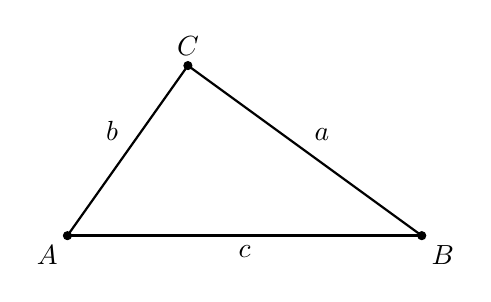
\begin{tikzpicture}[scale=0.9,>=stealth]
  \coordinate (P) at (0,0);
  \coordinate (Q) at (5,0);
  \coordinate (R) at (1.7,2.4);
  \draw[very thick] (P) -- (Q);
  \draw[thick] (P) -- (R) -- (Q);
  \foreach \p in {P,Q,R} \draw[fill] (\p) circle (1.6pt);
  \node[below left] at (P) {$A$};
  \node[below right] at (Q) {$B$};
  \node[above] at (R) {$C$};
  \node[below] at (2.5,0) {$c$};
  \node[above left] at (0.85,1.2) {$b$};
  \node[above right] at (3.35,1.2) {$a$};
\end{tikzpicture}
\end{center}

ইন্টুইশনটা সরল: $A$ থেকে $B$-তে যাওয়ার সবচেয়ে ছোট পথ হলো সরলরেখাংশ $AB$, আর
$C$ ঘুরে যাওয়া মানে একটি ঘুরপথ। সাবধান, ``দুই বিন্দুর মধ্যে সরলরেখাই সংক্ষিপ্ততম
পথ'' কথাটি আমরা এখানে \emph{প্রমাণ করছি না}; এটি ইউক্লিডীয় দূরত্বের একটি মৌলিক
ধর্ম হিসেবে ধরে নিচ্ছি। এটুকু স্পষ্ট করে বলে রাখা দরকার, কারণ এই সিরিজের নিয়ম
হলো যা প্রমাণ করা হয়নি তা যেন ধরে-নেওয়া বলেই চিহ্নিত থাকে।

সংখ্যার জগতে এই একই ধারণা পরম মান দিয়ে লেখা হয়, এবং সেই রূপটি আমরা পুরোপুরি
প্রমাণ করতে পারি।

\begin{idea}[পরম মান]
বাস্তব $x$-এর পরম মান
\[
  |x| = \begin{cases} x, & x \geq 0 \\ -x, & x < 0 \end{cases}
\]
অর্থাৎ $|x|$ হলো সংখ্যারেখায় $0$ থেকে $x$-এর দূরত্ব, আর $|x - y|$ হলো $x$ ও
$y$-এর মধ্যেকার দূরত্ব। মূল ধর্মগুলো: $|x| \geq 0$; $|xy| = |x||y|$;
$-|x| \leq x \leq |x|$; এবং $c > 0$ হলে
\[
  |x| \leq c \iff -c \leq x \leq c .
\]
একইভাবে $c > 0$ হলে $|x| \geq c$ হওয়ার শর্ত হলো $x \geq c$ অথবা $x \leq -c$।
\end{idea}

\begin{idea}[ত্রিভুজ অসমতা, পরম মানের রূপ]
যেকোনো বাস্তব $a, b$-এর জন্য
\[
  |a + b| \;\leq\; |a| + |b| ,
\]
এবং সমতা ঘটে কেবল তখন, যখন $a$ ও $b$ একই চিহ্নের (বা তাদের একটি শূন্য)।
\end{idea}

প্রমাণ: $-|a| \leq a \leq |a|$ এবং $-|b| \leq b \leq |b|$, এই দুটি অসমতা যোগ
করলে
\[
  -\left( |a| + |b| \right) \;\leq\; a + b \;\leq\; |a| + |b| .
\]
এখন উপরের ধর্মটি $c = |a| + |b|$ নিয়ে উল্টো দিকে পড়লে $|a+b| \leq |a| + |b|$।
সমতা যাচাই করতে দুই পাশ বর্গ করা সুবিধাজনক: $(a+b)^2 \leq (|a|+|b|)^2$ মানে
$2ab \leq 2|a||b| = 2|ab|$, আর সমতা ঘটে ঠিক তখনই যখন $ab = |ab|$, অর্থাৎ
$ab \geq 0$।

\begin{example}
সমাধান করো: (ক) $|x - 4| < 3$; (খ) $|2x + 3| \geq 5$।
\end{example}

\begin{solbox}
(ক) $|x-4| < 3$ মানে $-3 < x - 4 < 3$, অর্থাৎ $1 < x < 7$। দূরত্ব হিসেবে পড়লে:
$4$ থেকে যেসব সংখ্যার দূরত্ব $3$-এর কম, তারাই সমাধান, অর্থাৎ ব্যবধি $(1,7)$।

(খ) $|2x+3| \geq 5$ মানে $2x + 3 \geq 5$ অথবা $2x + 3 \leq -5$। প্রথমটি থেকে
$x \geq 1$, দ্বিতীয়টি থেকে $x \leq -4$। সমাধান
$(-\infty, -4] \cup [1, \infty)$।
\end{solbox}

\begin{example}
প্রমাণ করো যে যেকোনো বাস্তব $a, b$-এর জন্য
$\bigl| \, |a| - |b| \, \bigr| \leq |a - b|$।
\end{example}

\begin{solbox}
$a$-কে একটু ঘুরিয়ে লিখি: $a = (a - b) + b$। ত্রিভুজ অসমতা প্রয়োগ করলে
\[
  |a| \leq |a-b| + |b| \;\Longrightarrow\; |a| - |b| \leq |a-b| .
\]
একইভাবে $b = (b-a) + a$ লিখে $|b| - |a| \leq |b-a| = |a-b|$। সুতরাং
$|a| - |b|$ রাশিটি $|a-b|$-এর চেয়ে বড় নয় এবং $-|a-b|$-এর চেয়ে ছোট নয়, অর্থাৎ
$\bigl| \, |a| - |b| \, \bigr| \leq |a-b|$।
\end{solbox}

\begin{remark}
এই অসমতাটি ২০ নম্বর অধ্যায়ে ভেক্টর আকারে ফিরে আসবে:
$|\mathbf{A} + \mathbf{B}| \leq |\mathbf{A}| + |\mathbf{B}|$। ভৌত অর্থ হলো, দুটি
বলের লব্ধির মান কখনোই তাদের মানের যোগফলকে ছাড়াতে পারে না, এবং সমতা ঘটে কেবল
তখনই, যখন বল দুটি একই দিকে কাজ করে।
\end{remark}

\prob{2} সমাধান করো: (ক) $|3x - 1| \leq 8$; (খ) $|5 - 2x| > 3$।

\begin{sol}
(ক) $-8 \leq 3x - 1 \leq 8$, অর্থাৎ $-7 \leq 3x \leq 9$, অর্থাৎ
$-\dfrac{7}{3} \leq x \leq 3$।

(খ) $5 - 2x > 3$ অথবা $5 - 2x < -3$। প্রথমটি থেকে $-2x > -2$, এবং ঋণাত্মক সংখ্যা
দিয়ে ভাগ করায় চিহ্ন উল্টে $x < 1$। দ্বিতীয়টি থেকে $-2x < -8$, অর্থাৎ $x > 4$।
সমাধান $(-\infty, 1) \cup (4, \infty)$।
\end{sol}

\prob{3} $a, b, c$ একটি ত্রিভুজের তিন বাহুর দৈর্ঘ্য হলে প্রমাণ করো যে
$|a - b| < c < a + b$।

\begin{sol}
ডান দিকের অসমতাটি ত্রিভুজ অসমতা নিজেই। বাম দিকের জন্য বাকি দুটি ত্রিভুজ অসমতা
ব্যবহার করি। $a < b + c$ থেকে $a - b < c$, আর $b < c + a$ থেকে $b - a < c$।
সুতরাং $a - b$ এবং $b - a$ দুটিই $c$-এর চেয়ে ছোট; এদের একটি হলো $|a-b|$।
অতএব $|a - b| < c$।
\end{sol}

\prob{4} $a, b, c$ একটি ত্রিভুজের তিন বাহুর দৈর্ঘ্য হলে প্রমাণ করো যে
\[
  \frac{a}{b+c} + \frac{b}{c+a} + \frac{c}{a+b} \;<\; 2 .
\]

\begin{sol}
ধরি $s = a + b + c$। ত্রিভুজ অসমতা অনুযায়ী $b + c > a$, তাই দুই পাশে $b+c$ যোগ
করলে $2(b+c) > a + b + c = s$, অর্থাৎ $b + c > \dfrac{s}{2}$। হর বড় হলে ভগ্নাংশ
ছোট হয় (নিয়ম ৫), সুতরাং
\[
  \frac{a}{b+c} \;<\; \frac{a}{s/2} = \frac{2a}{s} .
\]
একইভাবে $\dfrac{b}{c+a} < \dfrac{2b}{s}$ এবং $\dfrac{c}{a+b} < \dfrac{2c}{s}$।
তিনটি যোগ করে
\[
  \frac{a}{b+c} + \frac{b}{c+a} + \frac{c}{a+b}
  \;<\; \frac{2(a+b+c)}{s} = 2 .
\]
লক্ষ করো, এখানে ত্রিভুজের শর্তটি সত্যিই দরকার ছিল; যেকোনো ধনাত্মক $a,b,c$-এর
জন্য দাবিটি সত্য নয়।
\end{sol}

\section{কোশি-শোয়ার্জ}

AM--GM যোগফল ও গুণফলের মধ্যে সেতু বাঁধে। পরের অসমতাটি সেতু বাঁধে দুই সারি
সংখ্যার মধ্যে, এবং পদার্থবিজ্ঞানে এটি এত ঘন ঘন আসে যে অনেকে না জেনেই এটি ব্যবহার
করে ফেলে। এখানে কেবল পরিচয় করিয়ে দেওয়া হচ্ছে; ভেক্টর হাতে এলে এর আসল চেহারা
ধরা পড়বে।

\begin{idea}[কোশি-শোয়ার্জ অসমতা]
যেকোনো বাস্তব $a_1, \dots, a_n$ ও $b_1, \dots, b_n$-এর জন্য
\[
  \left( \sum_{i=1}^{n} a_i b_i \right)^{2}
  \;\leq\; \left( \sum_{i=1}^{n} a_i^2 \right)
           \left( \sum_{i=1}^{n} b_i^2 \right) .
\]
সমতা ঘটে কেবল তখন, যখন দুটি সারি সমানুপাতিক, অর্থাৎ কোনো ধ্রুবক $\lambda$-এর
জন্য সব $i$-তে $b_i = \lambda a_i$ (অথবা সব $a_i = 0$)।
\end{idea}

$n = 2$-এর ক্ষেত্রে প্রমাণটি একটি অভেদমাত্র, যা তুমি হাতে গুণ করেই যাচাই করতে
পারো:
\[
  (a^2+b^2)(x^2+y^2) - (ax+by)^2 \;=\; (ay - bx)^2 .
\]
ডান পাশ একটি বর্গ, তাই অঋণাত্মক; সুতরাং $(ax+by)^2 \leq (a^2+b^2)(x^2+y^2)$,
এবং সমতা ঠিক তখনই যখন $ay = bx$, অর্থাৎ $(a,b)$ ও $(x,y)$ সমানুপাতিক।

সাধারণ $n$-এর জন্য একটি কৌশল লাগে, যেখানে ৩ নম্বর অধ্যায়ের পূর্ণবর্গ
সম্পূর্ণ করার কায়দাটি কাজে লাগে। যেকোনো বাস্তব $t$-এর জন্য বিবেচনা করো
\[
  f(t) = \sum_{i=1}^{n} (a_i t + b_i)^2 = A t^2 + 2Bt + C ,
\]
যেখানে $A = \sum a_i^2$, $B = \sum a_i b_i$ এবং $C = \sum b_i^2$।
$f(t)$ বর্গের যোগফল, তাই সব $t$-এর জন্য $f(t) \geq 0$। যদি $A = 0$ হয়, তবে সব
$a_i = 0$ এবং অসমতাটি স্পষ্টভাবেই সত্য ($0 \leq 0$)। তাই ধরি $A > 0$ এবং পূর্ণবর্গ
সম্পূর্ণ করি:
\[
  f(t) = A\left( t + \frac{B}{A} \right)^{2} + \left( C - \frac{B^2}{A} \right) .
\]
এখন $t = -B/A$ বসালে প্রথম পদটি মুছে যায় এবং বাকি থাকে $C - B^2/A$। যেহেতু
$f(t) \geq 0$ সব $t$-এর জন্য, তাই $C - B^2/A \geq 0$, অর্থাৎ $B^2 \leq AC$।
এটিই কোশি-শোয়ার্জ। সমতা পেতে হলে ওই $t$-এ $f(t) = 0$ হতে হবে, অর্থাৎ প্রতিটি
$a_i t + b_i = 0$ হতে হবে, যা ঠিক সমানুপাতিকতার শর্ত।

\begin{example}
$x + 2y = 10$ হলে $x^2 + y^2$-এর ক্ষুদ্রতম মান নির্ণয় করো।
\end{example}

\begin{solbox}
সারি দুটি নাও $(1, 2)$ এবং $(x, y)$। কোশি-শোয়ার্জ বলছে
\[
  (1 \cdot x + 2 \cdot y)^2 \;\leq\; (1^2 + 2^2)(x^2+y^2) ,
\]
অর্থাৎ $100 \leq 5(x^2+y^2)$, সুতরাং $x^2 + y^2 \geq 20$। সমতার শর্ত হলো
$(x,y)$ ও $(1,2)$ সমানুপাতিক, অর্থাৎ $y = 2x$; শর্তে বসিয়ে $x + 4x = 10$, তাই
$x = 2$ ও $y = 4$। তখন $x^2+y^2 = 4 + 16 = 20$, অর্থাৎ সীমাটি সত্যিই অর্জিত হয়
এবং ক্ষুদ্রতম মান $20$।
\end{solbox}

\begin{remark}
২০ নম্বর অধ্যায়ে দেখা যাবে যে $\sum a_i b_i$ আসলে দুটি ভেক্টরের dot product
এবং $\sqrt{\sum a_i^2}$ তাদের দৈর্ঘ্য; তখন এই অসমতাটি দাঁড়াবে
$|\mathbf{a} \cdot \mathbf{b}| \leq |\mathbf{a}||\mathbf{b}|$, যার কারণ
$\mathbf{a} \cdot \mathbf{b} = |\mathbf{a}||\mathbf{b}| \cos\theta$ এবং
$|\cos\theta| \leq 1$। অর্থাৎ উপরের বীজগাণিতিক কসরতটুকু আসলে একটি কোণের কথাই
বলছিল। এই অনুচ্ছেদে তাই কোনো সমস্যা রাখা হয়নি; পরিচয়টুকুই যথেষ্ট।
\end{remark}

\section{চরম মান নির্ণয়}

এবার আসল লাভের জায়গা। ক্যালকুলাস ছাড়াই কীভাবে কোনো রাশির সর্বোচ্চ বা সর্বনিম্ন
মান বের করা যায়, তার একটি পূর্ণাঙ্গ পদ্ধতি অসমতা থেকে পাওয়া যায়।

\begin{idea}[সীমা প্লাস অর্জন]
$f$-এর ক্ষুদ্রতম মান $M$ প্রমাণ করতে দুটি কাজ লাগে, একটি করলে হবে না:
\begin{enumerate}
  \item গ্রহণযোগ্য সব ইনপুটের জন্য দেখাতে হবে $f \geq M$;
  \item অন্তত একটি ইনপুট দেখাতে হবে যেখানে $f$-এর মান ঠিক $M$।
\end{enumerate}
বৃহত্তম মানের জন্যও একই কথা, কেবল অসমতার মুখ উল্টো।
\end{idea}

\begin{remark}
দ্বিতীয় ধাপটি বাদ দেওয়া এই বিষয়ের সবচেয়ে সাধারণ ভুল। $x > 0$-এর জন্য
$x + \dfrac{9}{x} \geq 1$ কথাটি সত্য, কিন্তু $1$ ক্ষুদ্রতম মান নয়, কারণ কোনো
$x$-এ মানটি $1$ হয় না। এই কারণেই AM--GM-এর সমতার শর্তটি এত গুরুত্বপূর্ণ:
সেটিই দ্বিতীয় ধাপটি হাতে ধরিয়ে দেয়। ``সমতার শর্তই আসল তথ্য বহন করে'' কথাটির
মানে এটাই।
\end{remark}

\begin{example}
একটি আয়তক্ষেত্রের পরিসীমা $P$ নির্দিষ্ট। তার ক্ষেত্রফল সর্বাধিক কত হতে পারে?
\end{example}

\begin{solbox}
বাহু দুটি $x$ ও $y$ হলে $2(x+y) = P$, অর্থাৎ $x + y = P/2$, আর ক্ষেত্রফল $xy$।
AM--GM প্রয়োগ করি:
\[
  \sqrt{xy} \;\leq\; \frac{x+y}{2} = \frac{P}{4}
  \;\Longrightarrow\; xy \;\leq\; \frac{P^2}{16} .
\]
সমতা ঘটে $x = y = P/4$-এ, অর্থাৎ আয়তক্ষেত্রটি বর্গক্ষেত্র হলে; আর তখন ক্ষেত্রফল
ঠিক $P^2/16$। সুতরাং সর্বোচ্চ ক্ষেত্রফল $P^2/16$। নির্দিষ্ট পরিসীমায় বর্গক্ষেত্রই
সবচেয়ে বেশি জায়গা ঘেরে।
\end{solbox}

\begin{example}
একটি প্রক্ষেপকের (projectile) পাল্লা $R = \dfrac{v^2 \sin 2\theta}{g}$, যেখানে
$v$ ও $g$ নির্দিষ্ট। কোন $\theta$-তে পাল্লা সর্বাধিক?
\end{example}

\begin{solbox}
পাল্লার সূত্রটি এখানে পদার্থবিজ্ঞান থেকে দেওয়া ধরে নিচ্ছি; আমাদের কাজ কেবল
সর্বাধিক মান বের করা। ৭ নম্বর অধ্যায় থেকে জানি $\sin$ ফাংশনের মান কখনোই $1$
ছাড়ায় না, অর্থাৎ $\sin 2\theta \leq 1$। যেহেতু $v^2/g > 0$,
\[
  R = \frac{v^2}{g} \sin 2\theta \;\leq\; \frac{v^2}{g} .
\]
সমতা ঘটে যখন $\sin 2\theta = 1$, অর্থাৎ $2\theta = 90^{\circ}$, অর্থাৎ
$\theta = 45^{\circ}$। এই কোণটি গ্রহণযোগ্য, তাই সর্বাধিক পাল্লা $v^2/g$।
এখানে কোনো ডেরিভেটিভ নেওয়া লাগেনি; একটি সীমা আর তার অর্জনের বিন্দু, ব্যস।
\end{solbox}

\begin{remark}
১৫ নম্বর অধ্যায়ে এই একই কাজ ডেরিভেটিভ দিয়ে করা হবে। তখন খেয়াল রেখো যে
দুটি পদ্ধতির চরিত্র আলাদা: ডেরিভেটিভ শূন্য হওয়া কেবল স্থানীয় (local) চরম মানের
ইঙ্গিত দেয় এবং সেটি সর্বোচ্চ না সর্বনিম্ন তা আলাদা করে যাচাই করতে হয়, অথচ
অসমতা থেকে পাওয়া সীমা সরাসরি সর্বজনীন (global), কারণ সেটি সব ইনপুটের জন্য একসঙ্গে
প্রমাণিত।
\end{remark}

\prob{3} $x, y > 0$ এবং $x + y = 12$ হলে $x^2 y$-এর বৃহত্তম মান নির্ণয় করো।

\begin{sol}
সরাসরি $x$, $y$-এর উপর AM--GM প্রয়োগ করলে $x^2y$ পাওয়া যায় না, কারণ গুণফলে
$x$ দুবার লাগবে। তাই $x$-কে দুটি সমান টুকরোয় ভাগ করি এবং তিনটি রাশি
$\dfrac{x}{2}, \dfrac{x}{2}, y$ নিয়ে কাজ করি। এদের যোগফল $x + y = 12$, তাই
\[
  \left( \frac{x}{2} \cdot \frac{x}{2} \cdot y \right)^{1/3}
  \;\leq\; \frac{\dfrac{x}{2} + \dfrac{x}{2} + y}{3} = \frac{12}{3} = 4 ,
\]
অর্থাৎ $\dfrac{x^2 y}{4} \leq 64$, সুতরাং $x^2 y \leq 256$। সমতার শর্ত
$\dfrac{x}{2} = y$, যা $x + y = 12$-এর সঙ্গে মিলিয়ে $x = 8$, $y = 4$ দেয়;
তখন $x^2y = 64 \cdot 4 = 256$। সুতরাং বৃহত্তম মান $256$।

কৌশলটি মনে রাখার মতো: গুণফলে যে রাশিটি একাধিকবার আছে, তাকে সেই সংখ্যক সমান
টুকরোয় ভেঙে নিলে যোগফলটি ধ্রুবক থাকে এবং সমতার শর্তও অর্থবহ হয়।
\end{sol}

\prob{4} একটি বদ্ধ নলাকার (cylindrical) কৌটার আয়তন $V$ নির্দিষ্ট। ভূমির
ব্যাসার্ধ $r$ ও উচ্চতা $h$ হলে মোট পৃষ্ঠতল $S = 2\pi r^2 + 2\pi r h$। দেখাও যে
$S$ সর্বনিম্ন হয় যখন $h = 2r$, এবং সেই সর্বনিম্ন মান নির্ণয় করো।

\begin{sol}
$V = \pi r^2 h$ থেকে $h = \dfrac{V}{\pi r^2}$, তাই
\[
  S = 2\pi r^2 + 2\pi r \cdot \frac{V}{\pi r^2} = 2\pi r^2 + \frac{2V}{r} .
\]
এখানে সরাসরি দুই চলকের AM--GM প্রয়োগ করলে সমতার শর্ত থেকে $h = 2r$ আসে না, কারণ
দ্বিতীয় পদটি আসলে দুটি সমান টুকরোর যোগফল হিসেবে দেখা উচিত। তাই তিনটি ধনাত্মক
রাশি $2\pi r^2$, $\dfrac{V}{r}$, $\dfrac{V}{r}$ নিয়ে তিন চলকের AM--GM প্রয়োগ
করি:
\[
  \frac{S}{3} = \frac{2\pi r^2 + \dfrac{V}{r} + \dfrac{V}{r}}{3}
  \;\geq\; \left( 2\pi r^2 \cdot \frac{V}{r} \cdot \frac{V}{r} \right)^{1/3}
  = \left( 2\pi V^2 \right)^{1/3} ,
\]
অর্থাৎ $S \geq 3 \left( 2\pi V^2 \right)^{1/3}$।

সমতার শর্ত $2\pi r^2 = \dfrac{V}{r}$, অর্থাৎ $V = 2\pi r^3$। এই মান
$h = \dfrac{V}{\pi r^2}$-এ বসালে
\[
  h = \frac{2\pi r^3}{\pi r^2} = 2r ,
\]
অর্থাৎ কৌটার উচ্চতা তার ব্যাসের সমান। যেহেতু যেকোনো নির্দিষ্ট $V$-এর জন্য
$r = \left( \dfrac{V}{2\pi} \right)^{1/3}$ নিলে এই শর্ত মেটে, সীমাটি অর্জিত হয়
এবং সর্বনিম্ন পৃষ্ঠতল $3 \left( 2\pi V^2 \right)^{1/3}$।
\end{sol}

\begin{remark}
শেষ দুটি সমস্যায় একই কৌশল দুবার এসেছে: AM--GM প্রয়োগের আগে পদগুলোকে এমনভাবে
ভেঙে সাজানো, যাতে গুণফল থেকে চলকটি বেরিয়ে যায় এবং কেবল ধ্রুবক থাকে। এটিই
অসমতা দিয়ে চরম মান বের করার কেন্দ্রীয় কৌশল। কোন ভাগে ভাঙতে হবে তা আগে থেকে বলা
যায় না; উল্টো দিক থেকে ভাবতে হয়, অর্থাৎ ``গুণফলে $r$ কাটাকাটি হয়ে যাক'' এই
শর্ত থেকে ভাগগুলো ঠিক করতে হয়।
\end{remark}

\end{document}
